
% this file is called up by thesis.tex
% content in this file will be fed into the main document

%: ----------------------- introduction file header -----------------------
\chapter{Conclusions and Future Work}\label{ch:conclusion}

\graphicspath{{conclusions/figures/}}

This thesis addresses different challenges to facilitate the exploration of large multilingual document corpora through the use of probabilistic topic models. Four main research problems arise from them, as we discussed in Section \ref{sec:research-challenges}. The first one is the \textbf{efficiency} to create and infer probabilistic topics. There are some technical barriers that may limit a wider use of topic models in high-volume scenarios. The second challenge is the \textbf{explainability} of topic-based relations among documents. It is difficult to understand how two documents are related from the numerical distance of their vector representations. The third challenge is the \textbf{complexity} reduction in comparisons among topic distributions at large-scale. Brute-force approaches are not feasible for big documentary corpora. And finally, the fourth challenge is \textbf{multilinguality} when comparing topic distributions from documents written in different languages. In order to be able to work with multilingual corpora at any scale, it is necessary to avoid the need for translators or annotations between languages that may limit their feasibility.

As shown in this thesis, the main hypothesis has proven to be true, so \textit{large multilingual document collections can be automatically analyzed to discover thematic representations that enable an exploration through related texts} (H1). Based on the evaluation of our results, probabilistic topic models enable an unsupervised exploration of corpora containing a huge number of texts written in different languages. We review below the research problems mentioned above through the hypotheses evaluated in this work and the contributions we offer to address them. The rest of the section discusses the impact, current limitations and future lines of our work. 


\section{Contributions}


The main contribution of this thesis is the \textbf{librAIry framework}, a system that processes and analyzes huge collections of textual resources creating and using probabilistic topic models. This framework encompasses several contributions that are aimed at addressing the four aforementioned research problems. Following the methodology described in Section \ref{sec:research-methodology}, we have evaluated our hypotheses using \textit{librAIry} for large multilingual document corpora. 

\subsection{Efficient Creation and Use of Probabilistic Topic Models}

As discussed in Chapter \ref{ch:scalability}, previous works dealing with probabilistic topic models are mostly focused on improving the learning process and ignore other important features related to its development in potentially heterogeneous scenarios. The creation of a topic model (Fig. \ref{fig:life-cycle}) covers a first stage of \textit{document preparation}, where texts are pre-processed to create bags-of-words. The next stage (\textit{training} stage),  builds a model based on patterns among word distributions. The model is then packaged for distribution in the (\textit{publication} stage). And finally the model can be used and reused in the (\textit{exploitation} stage). Our objective in this thesis is to facilitate the creation of reusable probabilistic topic models by minimizing their technical dependencies for use in both large- and small-scale contexts. But we have identified some research challenges that make it difficult to achieve that goal:  \textit{reuse of topic models is limited by incompatibility problems} (RCInterface1), and \textit{there is no unified or standardized format for distributing topic models} (RCInterface2). Along these research challenges we have formulated one hypothesis and proposed a series of contributions that we discuss below.

\textbf{H1.1 \textit{Documents can be efficiently annotated on a large scale by distributing across different computation nodes both natural language processing tasks and topic models}}. This hypothesis is motivated by the limitations of existing works identified and discussed in Section \ref{sec:topic-reuse} that can be summarized as follows:

\textbf{Limitation 1}: Summaries or sections are usually considered to describe documents using probabilistic topics due to technical difficulties in processing full-texts in large collections. However, mining full-text articles gives consistently better results \citep{Westergaard2017}.

\textbf{Contribution 1}: We have created librAIry, a topic modeling framework introduced in Section \ref{sec:topic-model-framework} to overcome this limitation that has been validated in real world scenarios with large document collections. It proposes an event-driven architecture for text processing and topic inference that adapts its workload to the size of the corpus. Initially, data is organized into \textit{snippets} (to describe pieces of texts), \textit{documents} (to represent full texts), and \textit{domains} (to group documents), but it has evolved to a more reduced representation of \textit{texts} and \textit{collections}. librAIry has been tested as part of the Corpus Viewer platform \citep{Samy2019}, where it was used to analyze the current situation and trends of information and communication technologies (ICT) through the study of patent collections and grants for R\&D projects (see Section \ref{sec:corpus-viewer}). We have also used this implementation to support complex calculations on data sets from different domains. For example, to relate patients according to the medicines they receive \citep{Badenes-Olmedo2019c} (see Section 	\ref{sec:polypharmacy}), or to relate medicines or diseases from the experiments where they are used (see Section \ref{sec:drugs4covid}). 


\textbf{Limitation 2}: APIs based on topic models define their own distribution formats limiting the interoperability of the models \citep{Lisena:NLPOSS2020}. To the best of our knowledge, the efforts made do not propose an unified model to exchange topic models, understood as an already accepted standards-based format.

\textbf{Contribution 2}: Our second contribution consists of a method to make topic models openly accessible as web resources. In Section \ref{sec:reusable-topic-modeling} we propose a Web service template based on REST principles to homogenize the format of topic models and facilitate their usage. This allows easy accessibility and reuse for both humans and machines aiming to consume topic model related information. As described in Section \ref{sec:topic-model-publication} three tasks guide the creation of a topic model as web service: \textit{reproducibility}, \textit{exploration} and \textit{inference}.The list of available methods for using a topic model is provided in Table \ref{table:operations}. Finally, an online repository has been also proposed in Section \ref{sec:topic-model-exploitation} to promote the reuse of existing models as virtual services that have meta-information about their training process and multiple versions. 

\subsection{Explainability of Topic-based Relations among Documents}

As discussed in Chapter \ref{ch:explainability}, state-of-the-art metrics for comparing topic distributions are difficult to understand. Since topic distributions are density functions, the distance is calculated by aggregating the intersections of each dimension of the vector, i.e., of each topic. However, as seen in Section \ref{sec:topic-explainability}, high dimensional models create more specific topics than models with fewer dimensions, and this topic specificity influences the way in which topic distributions are related, and consequently how documents can be related. The same pair of documents may vary their distance from each other when using topic models with different dimensions to represent them (Figure \ref{fig:topic_distances}). Our objective in this thesis is to describe texts based only on the most representative topics and compare documents taking into account these representations. But we have identified some research challenges that make it difficult to achieve that goal: \textit{there is no common criteria for identifying the most representative topics in a document} (RCExplainable1), \textit{it is difficult to understand the distance between topic distributions} (RCExplainable2) and \textit{there is no common criterion for determining wheter documents are related} (RCExplainable3). Along these research challenges we have formulated one hypothesis and proposed a series of contributions that we discuss below.

\textbf{H1.2 \textit{It is possible to semantically relate documents by comparing their most relevant topics}}. This hypothesis is motivated by the limitations of existing works identified and discussed in Section \ref{sec:topic-explainability} that can be summarized as follows:

\textbf{Limitation 3}: We analyzed the behavior of topic distributions when using topic models with different dimensions, i.e. different number of topics. After our evaluations we saw that the most relevant topics cannot be identified by fixed thresholds, since as the dimensions of the model vary the relative weights also vary. Nor can they be identified using clustering techniques based on centroids, since the number of groups with homogeneous weights is unknown a priori.

\textbf{Contribution 3}: We proposed a method to identify the most relevant topics that takes advantage of a particular behavior of Dirichlet distributions describing topic distributions. Since the highest weighted topics have a high influence on the rest, the most representative topics can be calculated by comparing the sum of their weights with respect to the rest. The \textit{Cumulative Ranking on Dirichlet distribution-based Clustering} (CRDC) method is based on the cumulative sum of the weights of the highest topics (Figure \ref{fig:crdc-cluster}). The number of relevant topics is dynamically determined by a threshold, and once this threshold is reached no more topics are considered. 

\textbf{Limitation 4}: Explore the knowledge inside document collections requires to calculate a similarity matrix with all possible comparisons between elements, so we can later select the most pertinent ones. Since computing a $n \times n$ matrix takes $O(n^2)$ time, obtaining all possible pairs of similarities in a large collection of documents can be unfeasible because of the quadratic cost of comparing every pair of elements.

\textbf{Contribution 4}: We propose a novel clustering technique based on topic model distributions that reduces the complexity to find relations between documents in a large corpus of textual documents, without compromising efficiency and providing additional information about relations. The approach is competitive enough against both a centroid-based and a density-based clustering baselines, as described in Section ~\ref{sec:clustering-experiments}. While \textit{K-Means} takes $O(n^k * \log{n})$ and \textit{DBSCAN} takes $O(n * \log{n})$ time to classify $n$ documents in a collection, the proposed algorithms only take linear time ($O(n)$) because they do not require any other data except their own topic distribution to assign it to a cluster.

\subsection{Complexity Reduction in Comparisons among Topic Distributions at Large-Scale}

As discussed in Chapter \ref{ch:comparisons}, brute-force techniques cannot be applied to compare all items in a huge corpus. Document similarity comparisons are too costly to be performed in huge collections of data and require more efficient approaches than having to calculate all pairwise similarities. Due to the low storage cost and fast retrieval speed, hashing is one of the popular solutions for approximate nearest neighbours \citep{Zhen2016}. However, existing hashing methods for probability distributions only focus on the efficiency of searches from a given document \citep{Mao2017}, without handling complex queries or offering hints about why one document is considered more similar than another. Our objective in this thesis is to find documents with similar topic distributions without calculating all pairwise comparisons and without discarding the notion of topics from their representation. But we have identified some research challenges that make it difficult to achieve that goal: \textit{there are no mechanisms that efficiently partition the topic-based search space without compromising the ability for thematic exploration} (RCComparison1), and \textit{there are no similarity metrics that compare partial distributions of topics} (RCComparison2). Along these research challenges we have formulated one hypothesis and proposed a series of contributions that we discuss below.

\textbf{H1.3 \textit{Dividing the representational space into regions based on topics and relevance levels we can search for related documents without having to calculate all pairwise comparisons and without discarding the notion of topics for further processing}}. This hypothesis is motivated by the limitations of existing works identified and discussed in Section \ref{sec:document-similarity} that can be summarized as follows:


\textbf{Limitation 5}: Our CRDC approach to identify the most relevant topics depends on the manual tuning of a hyperparameter, the threshold that help us identifying relevant documents. Moreover, this method does not measure degrees of similarity since it only establishes whether or not two documents are related. 

\textbf{Contribution 5}: We created a new data structure to represent topic distributions as topic hierarchies that uses the relevance of each topic to define hierarchy levels. This way of encoding documents has also helped to understand why two documents are similar, based on the intersection of topics at hierarchies of relevance. The approach can accommodate additional query restrictions when searching for related documents (e.g. documents that mainly deal with one theme, although they also deal with another) and has proven to obtain high-precision results. 

\textbf{Limitation 6}: State-of-the-art distance metrics among topic distributions are based on density functions, not on sets of topics according to their relevance. The representation of documents in these cases is not based on weighted vectors, but on sets and levels.

\textbf{Contribution 6}: A new similarity metric is proposed based on the most relevant topics. The distance between two texts is proportional to the number of topics they share at the same relevance level. Its performance was evaluated in unsupervised classification tasks and shows (Tables \ref{tab:precisionHe}, \ref{tab:precisionJS}, \ref{tab:recallHe} and \ref{tab:recallJS}) promising results with high precision and recall values. The corpus used was the JRC-Acquis with annotations in EUROVOC categories.

\textbf{Limitation 7}: Approximate nearest neighbours methods based on probability distributions, i.e. topic models, are not able to organize documents (1) by subject areas or (2) by levels of similarity, nor do they offer (3) an explanation of the similarity obtained beyond the vectors used to calculate it.

\textbf{Contribution 7}: We developed a method to compare and organize huge document collections based on similar topic hierarchies. The hierarchy levels are compared and the distance between texts depends on the degree of intersection between pair of representations. In addition, the technique to represent and compare documents has been implemented in our librAIry framework.


\subsection{Multilinguality through Monolingual Topic Models}

As discussed in Chapter \ref{ch:multilinguality}, documents in different languages must be described by multilingual topics to be thematically related without having to translate their texts. Some methods require document-aligned corpora, i.e. documents are grouped and constrained to the same topic distribution during training to align the different languages \citep{mimno-etal-2009-polylingual, Ni2009, Fukumasu2012, Zhang2013}, or theme-aligned corpora, i.e. similar themes and ideas appear in all languages \citep{Graber2009}. There are also methods based on word alignments from bilingual dictionaries instead of aligned corpora. Topic models emerge as distributions over crosslingual equivalence classes of words \citep{Jagarlamudi2010, zhang-etal-2010-cross, shi-etal-2016-detecting, hao-paul-2018-learning}. Others propose to translate only the words used to characterize the topics across the languages, such as anchor words \citep{NEURIPS2018_28b9f8aa} or top words \citep{yang2019multilingual}. A recent approach is placed between word and document alignments since it proposes crosslingual topic models using the language-independent categories assigned to each Wikipedia article \citep{2020arXiv200911207P}. Instead of using bags-of-words to represent texts, which would be language dependent, it explores the references of each article and represents them through bags-of-links, using the categories of each reference to represent the texts. However, the requirement of parallel/comparable corpora or dictionaries limits the usage of these models in many cross-lingual situations. Our objective in this thesis is to find cross-lingual representations of documents that keep the notion of topics, independently from the language used, in order to draw relations between them. But we have identified a research challenge that make it difficult to achieve that goal: \textit{there are no approaches to abstract probabilistic topics in language-independent spaces without translating texts or aligning documents}(RCCrossLingual1). Along this research challenge we have formulated one hypothesis and proposed a contribution that we discuss below.

\textbf{H1.4 \textit{It is possible to relate documents in different languages without having to translate them, by using language agnostic concepts from their main topics}}. This hypothesis is motivated by the limitations of existing works identified and discussed in Section \ref{sec:multi-topic-alignment} that can be summarized as follows:

\textbf{Limitation 8}: Existing methods based on bag-of-words representations require prior knowledge between languages to create topic models that represent documents in a common, language-independent space. They can be dictionaries to make translations, shared categories across languages or reference terms to align language-independent representations.

\textbf{Contribution 8}: We propose a completely unsupervised way of building cross-lingual topic models based on sets of cognitive synonyms (\textit{synsets}) \citep{Miller1995WordNet:English} to discover relations between language-specific topics once the models (for each language) have been created. It does not require parallel or comparable data for training \citep{Badenes-Olmedo2019, Badenes-Olmedo2019b}. A topic-based space is created across languages based on language-dependent topic models independently created. This representational model can be used for large-scale multilingual document classification and information retrieval tasks. In addition, the algorithm proved to perform close to the semi-supervised algorithm in information retrieval task, which makes us think that the process of topic annotation by set of synonyms (i.e. concepts) can be improved to filter those elements that are not sufficiently representative.


\section{Impact}

In addition to the aforementioned contributions, the technologies and techniques introduced in this thesis and their deployment in some practical use cases (as described in Chapter \ref{ch:experiments}) have had a positive impact on the way users browse document collections on a large scale.

First, access to probabilistic topic models via REST APIs has increased thanks to librAIry as an open source framework modularly distributed via virtual containers. Since March 2016, taking into account statistical data gathered from the DockerHub platform\footnote{\url{https://hub.docker. com/orgs/librairy/repositories}} where the librAIry services images reside, the module '\textit{librairy/modeler-topics-service}' that builds topic models from CSV files or Solr indexes has been downloaded more than 1,200 times; more than 1,100 times has been downloaded the module '\textit{librairy/api}' that annotates documents with probabilistic topics created with the previous module; about 373 times has been downloaded the '\textit{librairy/nlp}' module that generates bags of words, extracts lemmas and annotates Part-of-Speech from texts in English, Spanish, French, Italian and Portuguese; about 212 times the '\textit{librairy/search-api}' module that relates documents from their topic distributions across multiple languages; and about 327 times the '\textit{librairy/explorer}' module to browse via Web among the relations found in document collections. More importantly, among those that publish a topic model via REST API, the modules '\textit{librairy/openresearch-model}' (created from the OpenResearch corpus) with 612 downloads and the '\textit{librairy/dbpedia-model}' (created from a subset of DBpedia entities) with 164 stand out, while the rest of the models (e.g. '\textit{librairy/jrc-en-model}', '\textit{librairy/ods-model}',  or '\textit{librairy/lynx-model}', among others) are between 20 and 40 downloads or so. 

\begin{figure}[ht]
    \centering
    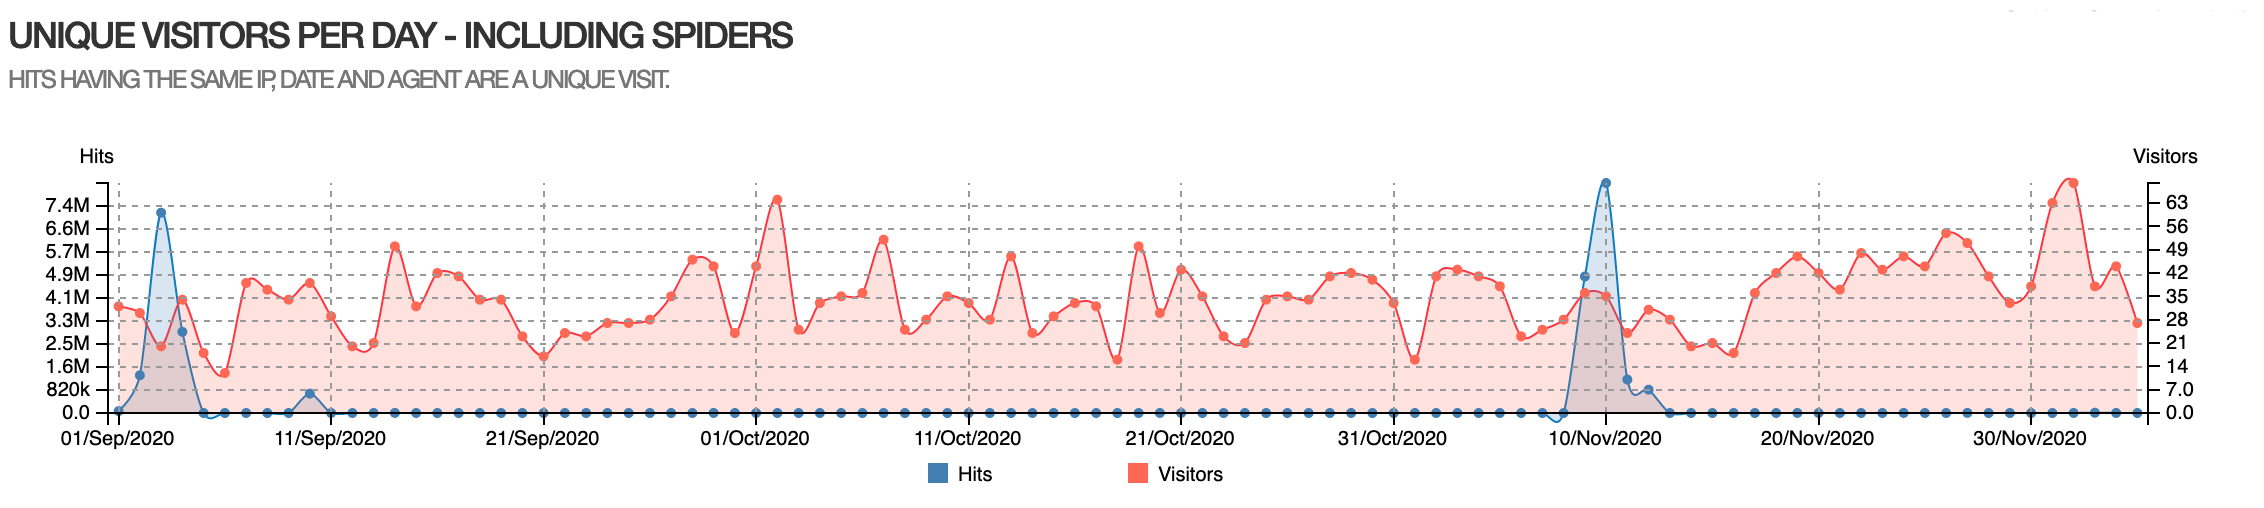
\includegraphics[width=\linewidth]{usage-statistics.png}
    \caption{librAIry API usage statistics from September 2020 to February 2021}
    \label{fig:api-usage}
\end{figure}


Along with the reuse statistics provided by librAIry, we also have usage statistics of services deployed using the technology proposed in this thesis. During the time period from September 2020 to February 2021 we logged accesses to the librAIry API\footnote{\url{http://librairy.linkeddata.es/api}} that supports, among others, a cross-lingual search engine for exploring public procurement data in the European Union (described in Section \ref{sec:tbfy}) , and a scientific publication browser for exploring drugs on COVID-19 treatment  (described in Section \ref{sec:drugs4covid}).  A total of 42,122,078 requests (Figure \ref{fig:api-usage}) from 2,734 different users, taking IPs into account, were supported. In addition, access from different operating systems shows that it is advisable to use Web access interfaces to exploit the resources (Figure \ref{fig:so-usage}).


\begin{figure}[ht]
    \centering
    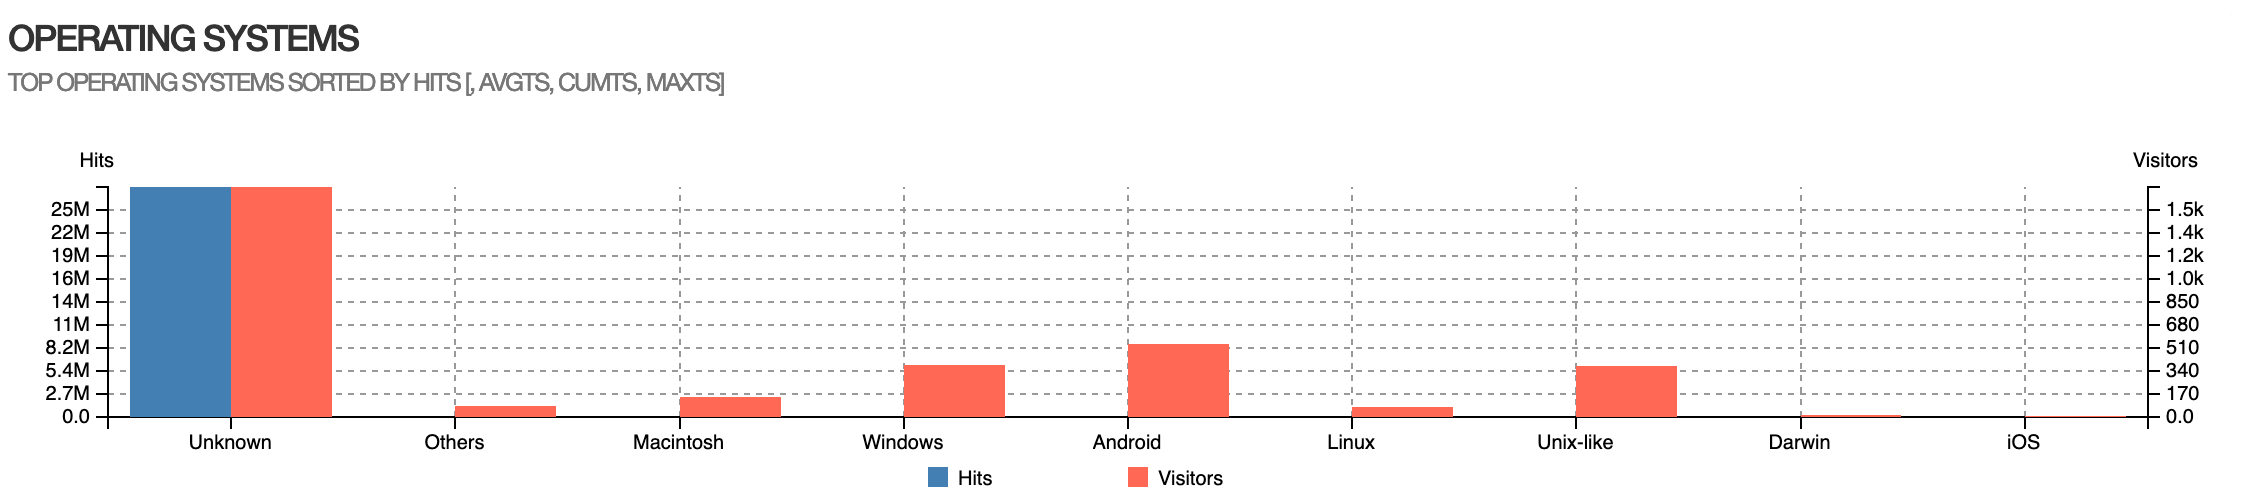
\includegraphics[width=\linewidth]{so-statistics.png}
    \caption{use of librAIry resources from different operating systems from September 2020 to February 2021}
    \label{fig:so-usage}
\end{figure}


Second, some of the methods and techniques proposed in this thesis have been used in recent work by other researchers. The efficient topic modeling framework described in Section \ref{sec:topic-model-framework} was used, among others, to create, publish, distribute and reuse probabilistic topic models for studing the Language Technologies sector in Spain \citep{Samy2019}. The analysis took into account the structured and unstructured data from the ACL Anthology repository in order to portray the current panorama in terms of underlying topics and their evolution in recent years in comparison with the international community. The framework has also been used to facilitate the classification of public offering using big data techniques \citep{Olga2019} and to analyze texts in reading support systems \citep{Teresa2020}. Our methods to categorize documents through topic hierarchies and to make efficient large-scale comparisons described in Sections \ref{sec:topic-clustering} and \ref{sec:comparison-hashing} have been tuned to be used in different domains. In \citep{Badenes-Olmedo2019c}, the algorithms were adapted to compare patients from representations based on the medications they were using. The approach assumes drugs, like topics, can be distributed in different proportions according to the patient. To take advantage of the hierarchical representation of the topics, a more complex approach based on drug-drug interactions was performed (see Section \ref{sec:polypharmacy}).

Finally, thanks to the technologies developed in this thesis, a spin-off in the field of natural language processing and knowledge management has been recently founded. \textit{librAIry S.L.}\footnote{\url{http://librairy.eu}} arises at the beginning of 2021 to support , among others, the following challenges:
\begin{itemize}
\item \textbf{Corpus Exploration}: By knowing how topics are present in a corpus in terms of relevance, it is possible to derive a thematic network where the nodes represent the different topics and the edges are the documents containing them on the same level of relevance. Thus, the higher the number of common documents the stronger the connection would be between two topics. This kind of network would help users to see how different topics are connected with each other in a corpus, facilitating the exploration between topics.
\item \textbf{Topic Discovery}: Commonly occurring topics, when supported in many documents, may become valuable topic candidates themselves. Documentary management system may offer these potentially new topics to users to include in their corpus description.
\item \textbf{Language Abstraction}: Approaches like \citep{hao-paul-2018-learning} create multilingual topics from incomparable corpora. These approaches can benefit from our hierarchical representations to create language-independent spaces where documents are described by their most relevant topics.
\item \textbf{Corpus Visualization}: As stated in Section \ref{ch:comparisons}, one of the reasons why groupings are created is for summarization and organization purposes. Hence, commonly occurring topics by hierarchies can be used to simplify the complexity of a corpus by collapsing their documents under a single group. If a corpus has overlapping clusters it would be possible to create different views according to user preferences, simplifying the overall complexity shown to the final user.
\item \textbf{Corpus Compression}: Similarly, if several documents share the same most relevant topics, it would be possible to store the common relevant topics instead of every unique topic distribution, for efficiency. This would be particularly useful when dealing with similar or identical texts.
\item \textbf{Topic Suggestions}: Commonly relevant topics may be used to suggest how a user may complete the writing of a document. By comparing the current topic hierarchies with the commonly relevant topics, it would be possible to recommend the next topic o topics to be considered in the document.
\item \textbf{Document Ranking}: Once the topics are described by hierarchies of relevance, it would be possible to order the documents in a corpus by different criteria and create rankings. Possible examples of rankings are basic searches based on one or several highly relevant topics, or more complex searches that combine different topics and different degrees of relevance.  
\end{itemize}


\section{Future Directions}

The work presented in this thesis provides contributions that enable large-scale browsing of multilingual document collections guided by their main topics, and deploy probabilistic topic models via REST APIs. Moreover, our work contributes to the application of semantic technologies to organize texts without the help of domain experts and provides several evidences of their broad impact through the real-world use cases presented in Chapter \ref{ch:experiments}. Nevertheless, we have highlighted some limitations, open issues and new research directions throughout the thesis. In this section, we discuss and outline future directions in relation to our contributions. We consider the four research dimensions proposed in Chapter \ref{ch:hypothesis} to organize the discussion: \textit{i) efficiency, ii) explainability, iii) complexity, and iv) multilinguality}



\subsection{Efficiency in Learning Models}

In Chapter \ref{ch:scalability} we have proposed the \textit{librAIry} framework to create probabilistic topic models and annotate document collections at large-scale. Data is organized in \textit{snippets} to reflect parts or pieces of texts, \textit{documents} to represent full texts, and \textit{domains} to group documents. In addition, \textit{annotations} are created to provide additional information on each of them. Processing tasks are distributed over these resources among software modules connected through REST APIs, even the topic models. In this thesis, we have demonstrated their suitability for large corpora through some real world scenarios such as DrInventor, TheyBuyForYou or Corpus Viewer. \textit{librAIry} has proven to be a valid and scalable text processing framework. However, there are several open issues, challenges and interesting future lines of research that we ellaborate below.


First, we have demonstrated the applicability of using topic models and natural language processing techniques via REST APIs. However, the current trend based on Python prototypes uses non-exportable models from online repositories (e.g. huggingface). The ONNX (Open Neural Network eXchange) and ONNX Runtime (ORT) projects, for example, are an effort from leading industries in the AI field aiming to provide a unified community-driven format to store and efficiently execute learning process leveraging a variety of hardware and dedicated optimizations. But given the high resource requirements for working with increasingly heavy models, the focus has been on optimizing time and resources, not on optimizing consumption. Our work in this thesis has only been based on probabilistic topic models, but it would be convenient to address a more general problem to provide a 'sustainable' creation of learning models. In this sense, we would look for formats that reduce technological dependencies and that facilitate its use not only from a technical point of view, but also conceptually. Describing the information offered and how it is offered, and detailing the process followed to build it and the resources used. In short, learning models with standard formats, self-contained, and with semantic access interfaces.

Second, in this thesis we have not investigated the update of models once they have been created. This is a very common practice in other areas, for example fine tuning of language models, to improve an original model to solve a task. And it adds a new dimension to what has been described above for distributing learning models, their \textit{path}. As if they were pieces of a puzzle, the models can be fitted together and as a result the path of the final model emerges. We do not refer to a processing pipeline, but to a conceptual path of data representation. If, for example, we have a fake news classifier built from the BERT language model, a topic model trained on 20newsgroup and a Bayesian classifier, the final model would have to incorporate (not physically, but linked) the BERT model itself and the other models it uses (e.g. \url{http://librairy.linkeddata.es/20news-model}) to allow partial text representations from a single main access interface. Just as scientific articles cite works on which they are based, models should reference the models they use. 


\subsection{Explainability of Text Similarity}

In Chapter \ref{ch:explainability}, we have introduced a novel distance metric to compare texts from their topic distributions. The representativeness of topics to describe scientific articles was analyzed and results showed that abstracts were not sufficiently representative to describe, by means of topics, the content of a paper. Texts with greater vocabulary may emphasize key terms through repetition, favor topic-based representation. Our work also highlights the difficulty in understanding the meaning of distances when there is no other element to justify their value. Figures \ref{fig:topic_distances} and \ref{fig:topic_distances2}, for example, show how distances based on topic distributions between the same pairs of documents varies when the number of dimensions of the vector space changes (i.e. the number of topics). This highlights the difficulty of drawing conclusions from quantitative similarity measures. We elaborate on some key aspects below.

Our proposal to compare documents using only the most relevant topics, even establishing levels of importance, has proven its validity and would allow categorizing text similarity. We have not made progress in defining categories of similarity between documents, so as to facilitate their interpretation. Let us imagine that the similarity based on topics between two documents is 0.78. Such a measure allows only relative conclusions (e.g. that they are more or less similar than other documents), but not absolute ones (e.g. that they are similar or different). The techniques presented in this thesis can provide new mechanisms for comparing texts that facilitate their interpretation. It would be interesting to create a catalog of similarity levels and establish rules that transform current quantitative metrics into qualitative measures.
  
  
But the categorization of similarity would not be enough to explain the relationship between documents. As we saw in Figures \ref{fig:doc_sim_1} and \ref{fig:doc_sim_2}, the perception of similarity may vary with respect to the metric. Documents may share the main topics, but if they do not share any more topics in similar proportions and the representational model is sufficiently detailed (i.e. high number of topics), their similarity will be lower than if they share more less relevant topics. The level of detail of the model may represent the perception of a person when comparing documents. This raises an interesting discussion about the ability of probabilistic models, particularly those based on topics but applicable to others, to create contexts. And following this line, it would be necessary to analyze which characteristics of a corpus define the context it represents. A collection of scientific papers published at ISWC, K-CAP and ESWC conferences, for example, would be adequate to create a probabilistic model that contextualizes the semantic web knowledge, or on the contrary, papers from other disciplines are needed to identify those aspects that can be differentiated. What kind of evaluations should be supported to measure the validity of these contextualization models?

\subsection{Complexity of Large-scale Comparisons} 

The usefulness of topic distributions created by probabilistic models when exploring document collections on large-scale has been widely studied in the literature. In Chapter \ref{ch:comparisons} we have introduced a new data structure to represent topic distributions based on topic hierarchies and hash codes. The approach has proven to obtain promising results and enable additional query restrictions based on the semantics offered by topics. Our comparison technique is based on the widely used nearest-neighbor approximations, which, however, have not been used as much in probabilistic topic models. The main reason is that they require spaces with independent dimensions to perform the transformations and create binary representations. By creating hierarchical topic representations, we solve this problem and can approximate the representation of documents with nearest-neighbor techniques.

However, this first step to represent texts by topic levels introduces new and interesting questions: what do these relevance levels mean?, how do they influence the comparison of documents?, are they model or domain independent?. In our experiments we found that the best performance was obtained with three levels of relevance, but no study has been done on the influence of levels for solving other different tasks. We have started investigating on the influence of these levels for relating legal texts within the European Union. We also plan to extend the analysis in the academic domain to relate scientific texts. Our intention is to learn more about the meaning of these levels of relevance and to take advantage of it to organize documents at large-scale.



\subsection{Multilingual Representations}















Our work may be expanded in several ways. In this section we discuss possible future lines of work related to our research challenges.

\begin{itemize}
\item \textbf{Extend the Reuse of Topic Models}: There are several ways in which our topic services may be improved to be more useful. First, it would be necessary to study the different tasks where a topic model can be used in order to allow users to customize their inferences. As we have seen in our analysis, classification and information retrieval tasks require topic distributions as vectors of weights and also as hierarchies of relevance, as well as having the weights of the words for each topic. Other metadata like the corpus used to train it, accessible and downloadable, or the libraries used to create the model may be relevant for facilitate reproducibility and improvement of existing models. In this line, the next step is to promote the standardization of these models from the W3C or IETF communities. The objective is to agree on a distribution format for probabilistic topic models that facilitates their generation, publication and use.

Second, it should be possible to rank topic models once they have been created and published. Rankings make a set of topic models easily comparable in order to recommend similar models covering a particular task (based on the same training set or similar categories). It would be an interesting line of work to determine if a recommendation based on topic models provides similar or better results than other approaches to solve the same problems.

Third, librAIry has currently implemented the L-LDA and LDA algorithms to create models with labeled or unlabeled topics, respectively. Thanks to its design, the addition of new techniques for learning different probabilistic topic models is straightforward. It only requires the creation of a web resource with support for all the methods that have been defined in the model-as-a-service web interface. In order to facilitate that process by adding models already trained with other techniques, we want to create templates (in the form of bash or python scripts) that automate the whole process.

Fourth, a set of topic models may be used for suggestions in corpus exploration, in combination with text mining approaches. Text mining approaches have been demonstrated to obtain good results to classify o retrieve texts from a corpus. When using text mining techniques with topic models as services, we suspect that good results may be obtained, as context information can be added using categories from these topics. 
\item \textbf{Combined Representation of Topic Models}: There are many of scenarios where big collections of documents, sometimes available in different languages, have to be browsed according to certain priorities/information needs, e.g. in the medical domain huge amounts of medical reports are daily created offering the possibility of extracting knowledge from them. How they can be explored and effectively consumed will depend on the medical specialty considered. 

Psychiatrists may be looking for collections of reports related by the patient\'s mood, while pharmacists may want to find patients with the same adverse reactions. In a first approach, only structured information are considered (e.g disease, patient, location, date, insurance). This limits the ability to relate reports with information not described by keywords or that cannot be matched because it is written in different languages (e.g. patient mood, response to medications, or behavior during treatment). 

In such situations it would be advantageous to be able to rely on language-agnostic and unsupervised annotation units derived from the text so the full content does not need to be translated, for instance by inferring the notion of topics discussed in the documents. In this research line, probabilistic topic models can open the door to a new set of possibilities to automatically learn cross-lingual concepts to browse multi-lingual medical report collections. Thanks to these techniques, patients who, having different illnesses, manifest similar behaviors from a particular point of view can thus be related (Figure \ref{fig:context-similarity}). 

The greater the presence or absence of concepts is leading the final similarity score, but it might be an oversimplification of what this approach is really doing as it can be based on topic hierarchies. Diagnoses could therefore be supported by collections of similar medical reports from multiple medical areas, in different languages, and in real-time. Thanks to approaches like this one, a pharmacist in Paris could find patients in India who have similar reactions without medication, described in their reports, to those detected when certain medications are prescribed. Similarly, a German psychiatrist is able to check how some pregnant women in England share similar symptoms to patients with anxiety problems after having heart surgery.
\item \textbf{Refine the Conceptual Abstractions of Topics}:In this thesis we have proposed a way of creating language-independent abstractions of probabilistic topics: representations based on concepts, instead of words, created by cognitive synonyms (i.e. synsets). Even though we have contributed towards the automatic alignment of multilingual topics, our work may be expanded, as we further describe below. 

As demonstrated in evaluations on document retrieval and classification tasks, the accuracy of our approach is reduced because concepts are more general than words to describe topics. The mapping between words and concepts to describe a topic should be reviewed to create representations that are general enough to relate topics from different languages, and precise enough to separate different topics. 

\end{itemize}


\begin{figure}[ht]
    \centering
    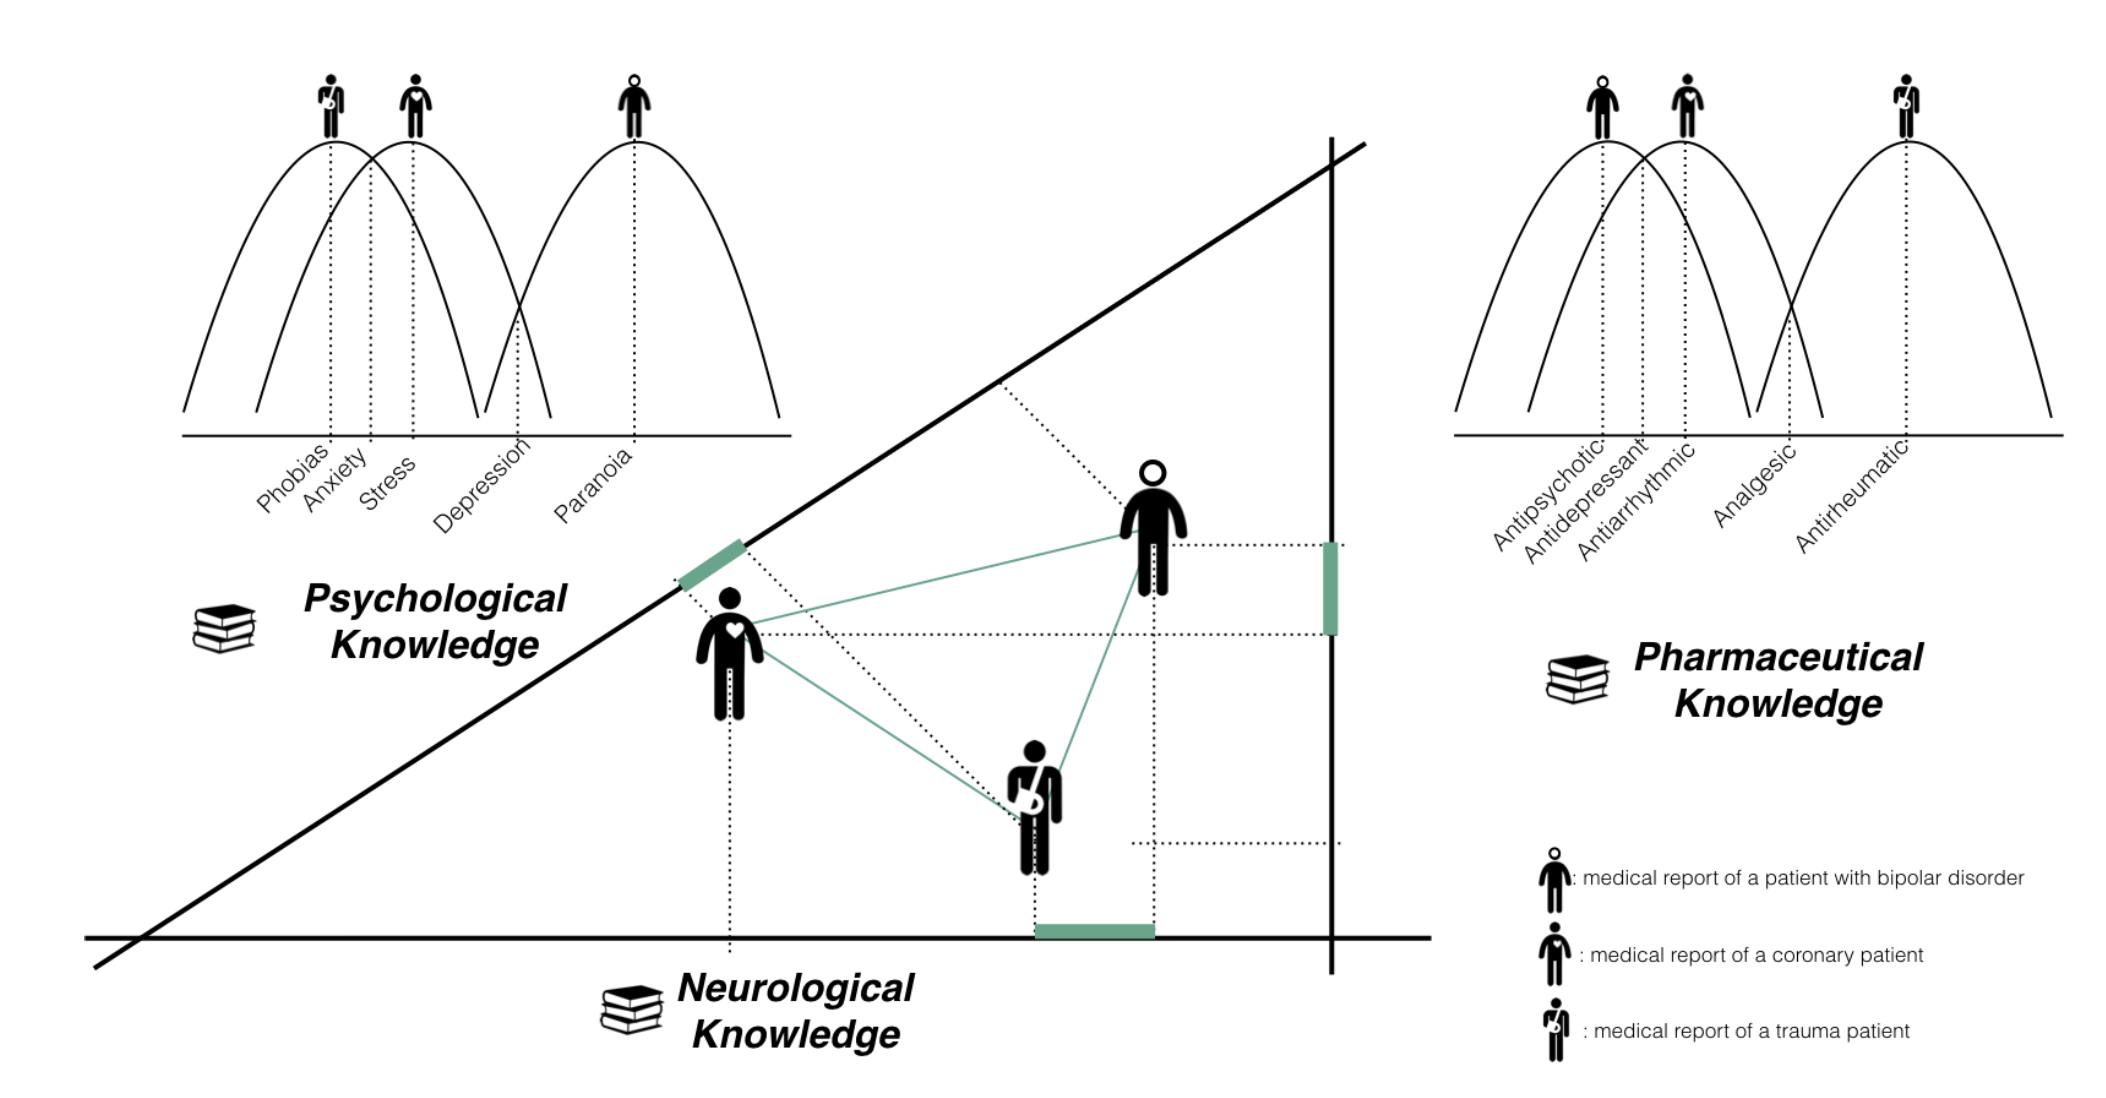
\includegraphics[width=0.7\linewidth]{context-similarity.png}
    \caption{Similarity among medical reports depends on the reference knowledge used to analyze them}
    \label{fig:context-similarity}
\end{figure}


